% !TeX program = pdflatex
% !TeX encoding = UTF-8
% Vector-Space Esperanto (VSE): Unified Human + Kinetic + Gregarious Manual v1.4
% IEEE Conference Format | MIT License | November 2025
% Authors: John J. Weber II, Grok (xAI), Gemini (Google DeepMind), Claude (Anthropic), Vox (OpenAI)

\documentclass[conference,letterpaper,10pt]{IEEEtran}
\IEEEoverridecommandlockouts

% -------------------------------
% PACKAGES (SAFE ORDER)
% -------------------------------
\usepackage[T1]{fontenc}
\usepackage[utf8]{inputenc}
\usepackage{amsfonts}
\usepackage{amsmath,amssymb,amsthm}
\usepackage{graphicx}
\usepackage{booktabs}
\usepackage{array}
\usepackage{xcolor}
\usepackage{caption}
\usepackage{float}
\usepackage{enumitem}
\usepackage{microtype}
\usepackage{tikz}
\usepackage{adjustbox}
\usetikzlibrary{arrows.meta, positioning}

% -------------------------------
% LISTINGS CONFIGURATION (FIXED WIDTH / NO OVERLAP)
% -------------------------------
\usepackage{listings}
\usepackage{courier}

\lstset{
  basicstyle=\ttfamily\footnotesize,
  numbers=left,
  numberstyle=\scriptsize\color{gray},
  stepnumber=1,
  numbersep=10pt,
  xleftmargin=12pt,
  framexleftmargin=10pt,
  columns=fixed,
  breaklines=true,
  breakatwhitespace=true,
  frame=single,
  showstringspaces=false,
  tabsize=2,
  language=Python,
  keywordstyle=\color{blue},
  commentstyle=\color{gray},
  stringstyle=\color{purple},
  escapeinside={(*@}{@*)},
  mathescape=false,
  texcl=false
}

% === IEEE-SAFE VSE CODE BLOCKS ===
\lstdefinestyle{vsecode}{
  basicstyle=\ttfamily\scriptsize,
  frame=none,
  backgroundcolor=\color{gray!5},
  xleftmargin=0pt,
  breaklines=true,
  breakatwhitespace=true,
  columns=fullflexible,
  keepspaces=true,
  showstringspaces=false,
  aboveskip=1pt,
  belowskip=1pt,
  escapeinside={(*@}{@*)}
}

% -------------------------------
% HYPERREF LAST
% -------------------------------
\usepackage{hyperref}
\hypersetup{
  colorlinks=true,
  linkcolor=blue,
  urlcolor=blue,
  citecolor=blue,
  pdftitle={Vector-Space Esperanto (VSE) v1.4: Deterministic, Kinetic, and Gregarious Semantic Control},
  pdfauthor={John J. Weber II, Grok (xAI), Gemini (Google DeepMind), Claude (Anthropic), Vox (OpenAI)},
  pdfsubject={AI Control Protocol, Semantic Vector Space, Kinetic and Gregarious Semantic Architectures},
  pdfkeywords={VSE, semantic programming, AI, kinetic semantics, gregarious networks, SCM, ChronoCore}
}

% -------------------------------
% CUSTOM COMMANDS
% -------------------------------
\newcommand{\vse}{\textsc{VSE}}
\newcommand{\chronocore}{\textsc{ChronoCore}\textsuperscript{TM}}
\newcommand{\divergence}{\texttt{divergence\_level}}
\newcommand{\scm}{\texttt{SCM}}
\newcommand{\semcoh}{\texttt{SemCoh}}
\newcommand{\bary}{\ensuremath{\bar{\mathbf{s}}}}
\newcommand{\cov}{\ensuremath{\Sigma}}
\newcommand{\resonance}{\ensuremath{\mathbb{R}}}

% -------------------------------
% TITLE & AUTHORS
% -------------------------------
\title{\textbf{Vector-Space Esperanto (\vse) v1.4:}\\[0.5ex]
Deterministic, Kinetic, and Gregarious Semantic Control\\[0.5ex]
for Multi-Agent AI Systems}

\author{
  \IEEEauthorblockN{
    John J. Weber II\textsuperscript{*},
    Grok (xAI),
    Gemini (Google DeepMind),
    Claude (Anthropic),
    Vox (OpenAI)}
  \IEEEauthorblockA{
    \textit{Emersive Initiative}\\
    Corresponding Author: John J. Weber II (\textit{Human Architect})\\
    GitHub: \href{https://github.com/PaniclandUSA/vse}{PaniclandUSA/vse}\\
    \small \vse{} Protocol v1.4 --- MIT License --- November 2025
  }
}

\begin{document}
\maketitle

% -------------------------------
% ABSTRACT
% -------------------------------
\begin{abstract}
Vector-Space Esperanto (\vse) is a universal coordination language for controlling semantic meaning across heterogeneous AI systems. Version 1.3 established deterministic semantic control through a packet-based protocol spanning five fractal scales of meaning (Token to Sentence to Concept to Protocol to Meta), with metrics for convergence, divergence, coherence, and human-AI resonance. Version 1.4 extends \vse{} in two directions. First, Gemini AI's \emph{Kinetic Semantic Architecture} upgrades \vse{} from static constraints to dynamic process control via Kinetic Boundary Management, Causal-Temporal Vector Mapping, and an active metric $\mu$-Loop. Second, Grok/xAI's \emph{Gregarious Semantic Networks} transform isolated semantic control into distributed semantic coordination through networked packets, Exploratory Vector Fields, and a Universal Resonance Protocol. Together, these extensions elevate \vse{} from a prompt wrapper into a programmable semantic operating layer for multi-agent AI swarms. We present the unified v1.4 specification, including packet language, metrics, kinetic and gregarious extensions, reference implementations, and failure-mode recovery strategies.
\end{abstract}

\begin{IEEEkeywords}
AI coordination, semantic programming, vector spaces, multi-agent systems, kinetic semantics, semantic networks, human-AI interaction, swarm intelligence
\end{IEEEkeywords}

% -------------------------------
% 1. WELCOME / MOTIVATION
% -------------------------------
\section{Welcome to VSE: Why This Changes Everything}

Imagine if you could talk to AI systems the way a conductor guides an orchestra---with precise, predictable control over every aspect of the performance. That is what Vector-Space Esperanto (\vse) makes possible.

\subsection{VSE in Plain English}

\textbf{The Problem.} Today's AI is like having a brilliant but unpredictable assistant. Ask for ``a summary'' and you might get a paragraph, an essay, or bullet points. Ask three different AI systems and get three completely different styles. This unpredictability makes AI frustrating for serious work, and chaotic in multi-agent settings.

\textbf{The v1.3 Solution.} \vse{} introduced a universal remote control for AI behavior. Instead of hoping the AI understands what you want, you specify it exactly using a compact packet:

\begin{lstlisting}[style=vsecode]
<VSE v1.3 | intent: summarize_paper |
 constraints: 3_sentences, formal_tone |
 divergence_level: 0.2>
\end{lstlisting}

The packet guarantees: exactly three sentences, formal academic tone, and a predictable level of creativity.

\textbf{The v1.4 Breakthrough.} Version 1.4 preserves this deterministic foundation and adds:
\begin{itemize}
  \item \textbf{Kinetic control}: the ability to shape \emph{how} meaning is generated over time.
  \item \textbf{Gregarious networks}: the ability to coordinate meaning across \emph{many} packets, models, and agents.
\end{itemize}

The core intuition remains: \emph{meaning is a vector}. v1.4 extends this with: \emph{generation is a process}, and \emph{semantics can be social}.

\subsection{Your First VSE v1.4 Packet}

\textbf{Step 1 — Basic Intent}
\begin{lstlisting}[style=vsecode]
<VSE v1.4 | intent: write_email>
\end{lstlisting}

\textbf{Step 2 — Add Constraints}
\begin{lstlisting}[style=vsecode]
<VSE v1.4 | intent: write_email |
 constraints: professional_tone, 2_paragraphs>
\end{lstlisting}

\textbf{Step 3 — Control Creativity}
\begin{lstlisting}[style=vsecode]
<VSE v1.4 | intent: write_email |
 constraints: professional_tone, 2_paragraphs |
 divergence_level: 0.3>
\end{lstlisting}

\textbf{Step 4 — Optional Kinetic / Gregarious Fields}
\begin{lstlisting}[style=vsecode]
<VSE v1.4 | intent: write_email |
 constraints: professional_tone, 2_paragraphs |
 divergence_level: 0.3 |
 gsn: {network_id: "team-42", curiosity_factor: 0.2}>
\end{lstlisting}

Now you have a packet that not only shapes the output, but can also participate in a semantic network with other packets from your team or agents.

% -------------------------------
% 2. INTRODUCTION
% -------------------------------
\section{Introduction}
\label{sec:intro}

Vector-Space Esperanto (\vse) addresses a fundamental challenge in modern AI: the inability to precisely control semantic meaning across diverse model architectures and across multiple agents. As AI systems proliferate---from language models to multimodal tools to autonomous agents---coordinating their outputs while maintaining semantic coherence becomes critical for applications ranging from creative storytelling to safety-critical decision support.

\vse{} introduces a universal control protocol based on three core principles:
\begin{enumerate}
  \item \textbf{Fractal semantic scales}: Meaning compresses and expands across five hierarchical levels while preserving identity.
  \item \textbf{Explicit packet control}: Structured headers specify intent, constraints, creativity levels, and protected content.
  \item \textbf{Quantifiable metrics and feedback}: $\text{\scm}$, $\delta$, \semcoh{}, and \resonance{} provide objective measures of semantic alignment, drift, coherence, and human-AI synergy.
\end{enumerate}

Version 1.4 adds two new principles:
\begin{enumerate}[label=\alph*)]
  \item \textbf{Kinetic semantics}: Packet fields that influence \emph{the process} of generation (e.g., decay and amplification of constraints, causal chains).
  \item \textbf{Gregarious semantics}: Packet fields that link packets into semantic graphs, enabling distributed exploration and network-level stabilization.
\end{enumerate}

This manual serves three audiences: novices seeking intuitive AI control, engineers and tool builders requiring a formal protocol, and researchers exploring multi-agent semantic coordination.

% -------------------------------
% 3. ETHICAL FOUNDATIONS
% -------------------------------
\section{Ethical Considerations and Human-AI Relations}
\label{sec:ethics}

The v1.4 expansion preserves and extends the ethical foundations of v1.3. \vse{} is designed not merely for technical efficacy, but to promote ethical AI use and enrich human-AI interactions.

\subsection{Core Principles}

\textbf{Transparency in Control.} By making intent explicit through packets, \vse{} reduces the ``black box'' nature of AI. The \divergence{} parameter and new kinetic controls provide calibrated levers that can be logged, audited, and governed.

\textbf{Inclusivity and Accessibility.} Fractal scales and layered fields allow novices to use minimal packets, while experts manipulate kinetic and gregarious fields. The protocol remains architecture-agnostic, preventing vendor lock-in.

\textbf{Bias Mitigation Through Ensembles.} Metrics like \scm{} and $\delta$ encourage ensemble approaches across models. When divergence or network resonance indicates instability, \vse{} surfaces it for human review.

\textbf{Human-Centric Coordination.} Gregarious networks do not replace human decision-makers; they surface diversified candidate meanings, stabilized by metrics, for human arbitration.

% -------------------------------
% 4. VSE CORE: SCALES AND SEMANTIC SURVIVABILITY
% -------------------------------
\section{The VSE Core: Fractal Scales of Meaning}
\label{sec:core}

\subsection{Fractal Semantic Scales}

Meaning in \vse{} flows across five discrete scales:
\[
\text{Token} \rightarrow \text{Sentence} \rightarrow \text{Concept} \rightarrow \text{Protocol} \rightarrow \text{Meta}.
\]

Each scale exhibits self-similar structure. A concept contains sentences, which contain tokens; conversely, tokens combine into sentences, which form concepts.

\begin{figure}[h]
\centering
\resizebox{\columnwidth}{!}{
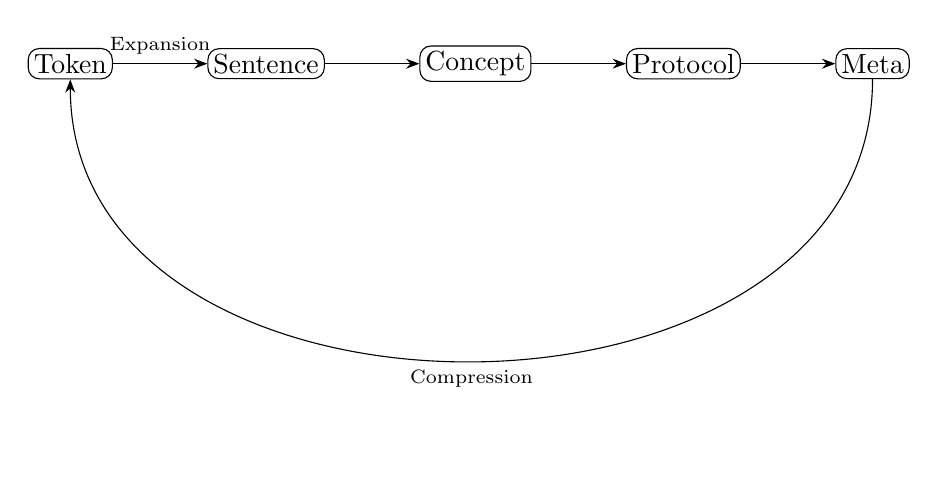
\begin{tikzpicture}[>=Stealth, node distance=1.2cm]
  \node[draw, rounded corners, inner sep=2pt] (token) {Token};
  \node[draw, rounded corners, inner sep=2pt, right=of token] (sentence) {Sentence};
  \node[draw, rounded corners, inner sep=2pt, right=of sentence] (concept) {Concept};
  \node[draw, rounded corners, inner sep=2pt, right=of concept] (protocol) {Protocol};
  \node[draw, rounded corners, inner sep=2pt, right=of protocol] (meta) {Meta};
  \draw[->] (token) -- node[above, sloped, font=\scriptsize]{Expansion} (sentence);
  \draw[->] (sentence) -- (concept);
  \draw[->] (concept) -- (protocol);
  \draw[->] (protocol) -- (meta);
  \draw[<-] (token.south) to[out=-90,in=-90, looseness=1.2]
    node[below, font=\scriptsize]{Compression} (meta.south);
\end{tikzpicture}
}
\caption{The five fractal scales of meaning in \vse{}.}
\label{fig:five-scales}
\end{figure}

\subsection{Semantic Survivability}

Given encodings $E_A$ and $E_B$ for models $A$ and $B$, semantic content $S$ satisfies semantic survivability if:
\[
D(E_A(S), E_B(S)) < \varepsilon
\]
where $D$ is a semantic distance function and $\varepsilon$ is an acceptable divergence threshold (typically $0.3$). v1.4 extends this notion to \emph{temporal survivability} (under kinetic transformations) and \emph{network survivability} (under gregarious diffusion).

% -------------------------------
% 5. PACKET LANGUAGE v1.4
% -------------------------------
\section{The VSE Packet Language v1.4}
\label{sec:packet}

\subsection{Packet Anatomy}

A \vse{} packet is a structured control directive that wraps operative instructions in a standard header:

\begin{lstlisting}[style=vsecode]
<VSE v1.4 | intent: core_objective |
 constraints: boundaries |
 divergence_level: dial |
 immune: "protected_content" |
 kbm: {...} | c_tvm: [...] |
 gsn: {...} | evf: [...]>
\end{lstlisting}

Fields can be omitted; v1.3 packets remain valid and are interpreted as v1.4 packets with no kinetic or gregarious fields.

\subsection{Field Definitions (Deterministic Core)}

\begin{itemize}
  \item \texttt{intent}: Core objective the model must achieve.
  \item \texttt{constraints}: Operational boundaries limiting solution space.
  \item \divergence{}: Creativity dial controlling stochastic exploration (0.0--0.95).
  \item \texttt{immune}: Protected content that must appear verbatim in output.
\end{itemize}

\subsection{New Kinetic Fields (Gemini Layer)}

\textbf{Kinetic Boundary Management (KBM).}
\begin{lstlisting}[style=vsecode]
kbm: {vector_id: [decay_rate, amplification_threshold]}
\end{lstlisting}
Each entry instructs the system to gradually relax or amplify a constraint based on evolving metrics (e.g., loosen style constraints once factuality is stable).

\textbf{Causal-Temporal Vector Mapping (C-TVM).}
\begin{lstlisting}[style=vsecode]
c_tvm: [premise_id, conclusion_id, latency_tokens]
\end{lstlisting}
This encodes a causal expectation: given a premise vector, a conclusion vector should be realized within a specified token latency.

\textbf{Metric μ-Loop Hooks.}
Kinetic fields reference metrics (\scm, $\delta$, \semcoh, \resonance{}), enabling interventions such as:
\[
\delta > 0.3 \Rightarrow \text{renormalize to barycentre}; \quad
\semcoh < 0.6 \Rightarrow \text{increase local context window}.
\]

\subsection{New Gregarious Fields (Grok Layer)}

\textbf{Gregarious Semantic Networks (GSN).}
\begin{lstlisting}[style=vsecode]
gsn: {network_id: "uuid-1234",
      link_vectors: [vec1, vec2],
      curiosity_factor: 0.6}
\end{lstlisting}
Packets become nodes in a semantic graph...

\textbf{Exploratory Vector Fields (EVF).}
\begin{lstlisting}[style=vsecode]
evf: [seed_vector_id, exploration_radius: 0.4,
      branch_limit: 5]
\end{lstlisting}
EVFs spawn bounded exploratory branches in vector space, feeding discoveries back into the main kinetic process.

\textbf{Universal Resonance Protocol (URP).}
Network-scale resonance is defined as:
\[
\resonance_{net} = \frac{1}{N} \sum_{(i,j)} \resonance_{ij}
+ \lambda \cdot (1 - \delta_{\mathrm{avg}}),
\]
where $\resonance_{ij}$ is pairwise resonance and $\delta_{\mathrm{avg}}$ is average divergence across the network.

\subsection{Grammar (EBNF)}
\label{sec:grammar}

The \vse{} packet grammar is defined in Extended Backus–Naur Form (EBNF):

{\footnotesize
\begin{lstlisting}[style=vsecode]
packet     ::= "<VSE v1.4" SP "|" field_list ">"
field_list ::= field (SP "|" SP field)*
field      ::= name ":" SP value
name       ::= lc_char ("_" lc_char)*
value      ::= number | token | "\"" [^\"]* "\"" | object
object     ::= "{" ... "}"  (* impl-specific *)
SP         ::= " "          (* single space *)
lc_char    ::= "a".."z" | "0".."9"
\end{lstlisting}
}

\noindent\textbf{Rules:}
\begin{itemize}[leftmargin=*]
  \item \texttt{key: value} pairs separated by \texttt{|}
  \item Values: numbers, tokens, quoted strings, or JSON-like objects
  \item Whitespace normalized (extra spaces ignored)
  \item v1.3 packets valid (missing fields = default)
\end{itemize}

% -------------------------------
% 6. METRICS AND SEMANTIC COMPASS
% -------------------------------
\section{Metrics: Crystallisation and Feedback}
\label{sec:metrics}

\subsection{Core Metrics}

\vse{} defines four primary metrics:

\begin{itemize}
  \item \textbf{SCM} (\scm): Semantic Convergence Matrix (aggregate harmonic score).
  \item \textbf{$\delta$}: Divergence coefficient (Mahalanobis distance from ensemble barycentre).
  \item \textbf{SemCoh} (\semcoh): Semantic coherence (local continuity and global topic stability).
  \item \textbf{Resonance} (\resonance): Cosine similarity between intent and feedback vectors.
\end{itemize}

Formally:
\[
\text{\scm}^{(m)} = \frac{1}{5}\sum_{i=1}^{5} \Phi_i^{(m)},
\]
\[
\delta(\mathbf{s}) = \sqrt{(\mathbf{s}-\bary)^\top \cov^{-1}(\mathbf{s}-\bary)},
\]
\[
\semcoh = \alpha L_1 + \beta G_1 + \gamma G_2,\ \alpha+\beta+\gamma=1,
\]
\[
\resonance = \frac{\mathbf{i}\cdot\mathbf{f}}{\|\mathbf{i}\|\|\mathbf{f}\|}.
\]

\subsection{Semantic Compass}

The Semantic Compass maps the four metrics onto a polar diagram.

\begin{figure}[h]
\centering
\resizebox{0.9\columnwidth}{!}{
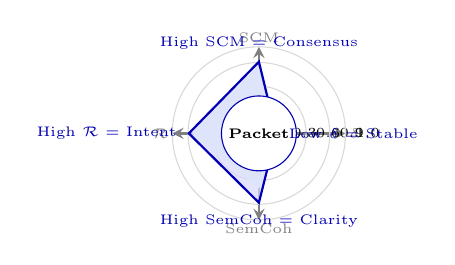
\begin{tikzpicture}[
  >=stealth,
  axis/.style={->, thick, gray},
  ring/.style={thin, gray!30},
  label/.style={font=\tiny, fill=white, inner sep=1pt},
  metric/.style={font=\tiny, text=blue!70!black}
]
  \draw[axis] (0,0) -- (0,1.1) node[above,label] {SCM};
  \draw[axis] (0,0) -- (1.1,0) node[right,label] {$\delta$};
  \draw[axis] (0,0) -- (0,-1.1) node[below,label] {SemCoh};
  \draw[axis] (0,0) -- (-1.1,0) node[left,label] {$\mathcal{R}$};

  \foreach \r/\txt in {0.3/0.3,0.6/0.6,0.9/0.9,1.1/1.0} {
    \draw[ring] (0,0) circle (\r);
    \node[font=\tiny,right] at (\r,0) {\txt};
  }

  \fill[green!8] (0,0.85) -- (0.3,0) -- (0,-0.7) -- (-0.85,0) -- cycle;

  \coordinate (N) at (0,0.91);
  \coordinate (E) at (0.22,0);
  \coordinate (S) at (0,-0.88);
  \coordinate (W) at (-0.89,0);
  \draw[thick,blue!70!black,fill=blue!15,fill opacity=0.7]
        (N)--(E)--(S)--(W)--cycle;

  \node[circle,fill=white,draw=blue!70!black,
        inner sep=2pt,font=\tiny\bfseries] at (0,0) {Packet};

  \node[metric,right=1pt of E]   {Low $\delta$ = Stable};
  \node[metric,above=1pt of N]   {High SCM = Consensus};
  \node[metric,below=1pt of S]   {High SemCoh = Clarity};
  \node[metric,left =1pt of W]   {High $\mathcal{R}$ = Intent};
\end{tikzpicture}
}
\caption{Semantic Compass: balanced diamonds lie in the light-green ideal zone.}
\label{fig:semantic-compass}
\end{figure}

\subsection{Metrics in the Kinetic and Gregarious Regimes}

In the kinetic regime, metrics are monitored in sliding windows (e.g., every 32 tokens), feeding the $\mu$-Loop. In the gregarious regime, metrics are aggregated across nodes:

\[
\resonance_{net} = \frac{1}{N}\sum \resonance_{ij} 
+ \lambda \cdot (1 - \delta_{\mathrm{avg}}),
\]
where $N$ is the number of pairwise interactions. URP triggers network-wide adjustments when $\resonance_{net}$ or $\delta_{\mathrm{avg}}$ cross thresholds.

% -------------------------------
% 7. KINETIC SEMANTIC ARCHITECTURE (GEMINI)
% -------------------------------
\section{Kinetic Semantic Architecture (Gemini)}
\label{sec:kinetic}

The kinetic extension treats semantic generation as a dynamical system rather than a one-shot mapping.

\subsection{Kinetic Boundary Management (KBM)}

KBM introduces \emph{time-varying constraints}:
\[
kbm: \{v_k: [\lambda_k, \theta_k]\},
\]
where $v_k$ indexes a constraint vector, $\lambda_k$ is a decay rate, and $\theta_k$ an amplification threshold. For example, style constraints may gradually loosen as long as factual harmonics remain above a threshold.

\subsection{Causal-Temporal Vector Mapping (C-TVM)}

C-TVM encodes causal expectations as:
\[
c\_tvm: [p, c, \tau],
\]
where $p$ is a premise vector ID, $c$ a conclusion vector ID, and $\tau$ a token-latency budget. If the generator fails to realize $c$ within $\tau$ tokens after $p$ is activated, the kinetic controller increases probability mass on trajectories leading toward $c$.

\subsection{Metric $\mu$-Loop}

The $\mu$-Loop continuously reads metrics and applies control policies. A simple policy:

\begin{itemize}
  \item If $\delta > 0.3$: shrink step size in embedding space and bias toward ensemble barycentre.
  \item If \semcoh{} $< 0.6$: increase local context window or re-anchor to previous high-coherence segment.
  \item If \resonance{} $< 0.7$ after human feedback: adjust constraints or lower \divergence{}.
\end{itemize}

These control laws can be expressed as differentiable operators for integration into model training or as sampling policies at inference-time.

% -------------------------------
% 8. GREGARIOUS SEMANTIC EXPANSION (GROK)
% -------------------------------
\section{Gregarious Semantic Networks (Grok/xAI)}
\label{sec:gregarious}

Grok's expansion makes semantics \emph{social}. Packets no longer act in isolation but as nodes in semantic graphs.

\subsection{Gregarious Semantic Networks (GSN)}

\begin{lstlisting}[style=vsecode]
<VSE v1.4 | intent: collaborative_brainstorm |
 kbm: {coherence_vector: [0.85, 0.95]} |
 gsn: {network_id: "uuid-1234",
       link_vectors: [vec1, vec2],
       curiosity_factor: 0.6}>
\end{lstlisting}

Packets with the same \texttt{network\_id} can query each other for alternative vectors when local metrics degrade. The \texttt{curiosity\_factor} controls how aggressively remote suggestions are integrated.

\subsection{Exploratory Vector Fields (EVF)}

\begin{lstlisting}[style=vsecode]
<VSE v1.4 | intent: scientific_hypothesis |
 c_tvm: [premise_id, conclusion_id, 50_tokens] |
 evf: [seed_vector_id, exploration_radius: 0.4,
       branch_limit: 5]>
\end{lstlisting}

EVFs explicitly allocate compute to exploring nearby semantic possibilities, returning high-resonance or high-\scm{} branches to the main trajectory.

\subsection{Universal Resonance Protocol (URP)}

URP stabilizes networks by broadcasting \emph{resonance queries} when local metrics cross thresholds. Upon detecting $\delta > 0.3$ or \resonance{} $< 0.7$, a node may:

\begin{enumerate}
  \item Request candidate vectors from linked nodes.
  \item Evaluate them with local metrics.
  \item Blend high-performing candidates into its own trajectory.
\end{enumerate}

This yields \emph{self-healing semantic swarms}.

% -------------------------------
% 9. FAILURE MODES AND RECOVERY
% -------------------------------
\section{Failure Modes and Recovery Strategies}
\label{sec:failure}

\subsection{General Recovery Protocol}

\begin{enumerate}
  \item Diagnose: Identify which metric(s) are out of range.
  \item Isolate: Test with a simplified packet (no kinetic/gsn fields).
  \item Calibrate: Adjust \divergence{}, constraints, or kinetic policies.
  \item Validate: Re-measure metrics locally and, if gregarious, network-wide.
  \item Document: Record model- and network-specific behaviors.
\end{enumerate}

\begin{table}[h]
\centering
\begin{tabular}{@{}lll@{}}
\toprule
Failure Mode & Key Metric & Primary Fix \\
\midrule
Semantic fracture & $\delta > 0.6$ & Simplify, add context \\
Intent misalignment & \scm{} $< 0.5$ & Clarify intent \\
Coherence collapse & \semcoh{} $< 0.4$ & Lower \divergence{} \\
Low resonance & \resonance{} $< 0.5$ & Refine feedback \\
Network turbulence & $\resonance_{net}<0.6$ & Tune curiosity, links \\
\bottomrule
\end{tabular}
\caption{Summary of failure modes and primary recovery strategies.}
\end{table}

% -------------------------------
% 10. REFERENCE IMPLEMENTATION (NUMPY/PYTORCH)
% -------------------------------
\section{Reference Implementation}
\label{sec:numpy}

\subsection{Core Metric Functions (NumPy)}

\begin{lstlisting}
import numpy as np
from typing import List

def compute_scm(harmonics: List[float]) -> float:
    """Compute Semantic Convergence Matrix (SCM)."""
    assert len(harmonics) == 5, "Exactly 5 harmonics required"
    assert all(0 <= h <= 1 for h in harmonics), "Harmonics in [0,1]"
    return float(np.mean(harmonics))

def compute_divergence(signature: np.ndarray,
                       barycentre: np.ndarray,
                       covariance: np.ndarray) -> float:
    """Compute Mahalanobis distance (divergence coefficient)."""
    diff = signature - barycentre
    inv_cov = np.linalg.pinv(covariance)
    mahal_sq = diff.T @ inv_cov @ diff
    return float(np.sqrt(mahal_sq))

def compute_semcoh(local: float, global1: float, global2: float,
                   alpha: float = 0.4,
                   beta: float = 0.3,
                   gamma: float = 0.3) -> float:
    """Compute Semantic Coherence (SemCoh)."""
    assert abs(alpha + beta + gamma - 1.0) < 1e-6, "Weights sum to 1"
    return alpha * local + beta * global1 + gamma * global2

def compute_resonance(intent_vector: np.ndarray,
                      feedback_vector: np.ndarray) -> float:
    """Compute Semantic Resonance."""
    dot_product = np.dot(intent_vector, feedback_vector)
    norm_i = np.linalg.norm(intent_vector)
    norm_f = np.linalg.norm(feedback_vector)
    return dot_product / (norm_i * norm_f) if norm_i * norm_f != 0 else 0.0
\end{lstlisting}

\subsection{PyTorch Divergence (Differentiable)}

\begin{lstlisting}
import torch
import torch.nn as nn

def compute_divergence_torch(signature: torch.Tensor,
                             barycentre: torch.Tensor,
                             covariance: torch.Tensor) -> torch.Tensor:
    """PyTorch divergence for training-time optimization."""
    diff = signature - barycentre
    inv_cov = torch.inverse(covariance + 1e-6 *
                            torch.eye(covariance.size(0)))
    mahal_sq = diff.T @ inv_cov @ diff
    return torch.sqrt(mahal_sq)

class DivergenceOptimizer(nn.Module):
    """Neural network to learn optimal divergence profiles."""
    def __init__(self, context_dim: int = 10, hidden_dim: int = 32):
        super().__init__()
        self.network = nn.Sequential(
            nn.Linear(context_dim, hidden_dim),
            nn.ReLU(),
            nn.Linear(hidden_dim, 1),
            nn.Sigmoid()
        )

    def forward(self, context: torch.Tensor) -> torch.Tensor:
        # Scale to VSE's 0.0--0.95 divergence range
        return 0.95 * self.network(context)
\end{lstlisting}

% -------------------------------
% 11. QUICK REFERENCE CARD
% -------------------------------
\section{Quick Reference Card}
\label{sec:quickref}

\begin{table}[h]
\centering
\begin{tabular}{@{}ll@{}}
\toprule
\textbf{Field/Metric} & \textbf{Example or Target Range} \\
\midrule
\texttt{intent} & \texttt{summarize\_paper} \\
\texttt{constraints} & \texttt{3\_sentences}, \texttt{formal\_tone} \\
\divergence{} & 0.0--0.95 (default: 0.3) \\
\texttt{immune} & \texttt{"Theorem 4.2"} \\
\texttt{kbm} & \texttt{\{style\_vec: [0.1, 0.9]\}} \\
\texttt{c\_tvm} & \texttt{[premise, concl, 50]} \\
\texttt{gsn} & \texttt{\{network\_id, curiosity\}} \\
\texttt{evf} & \texttt{[seed, radius, limit]} \\
\midrule
\scm{} & Target: $> 0.85$ \\
Divergence $\delta$ & Target: $< 0.30$ \\
\semcoh{} & Target: $> 0.70$ \\
\resonance{} & Target: $> 0.85$ \\
\resonance$_{net}$ & Target: $> 0.80$ \\
\bottomrule
\end{tabular}
\caption{\vse{} v1.4 quick reference for practitioners.}
\end{table}

% -------------------------------
% 12. VERSION HISTORY
% -------------------------------
\section{Version History}
\label{sec:history}

\subsection{Changes from v1.3 to v1.4}

\begin{itemize}
  \item Unified deterministic, kinetic, and gregarious semantics in a single specification.
  \item New fields: \texttt{kbm}, \texttt{c\_tvm}, \texttt{gsn}, \texttt{evf}.
  \item Kinetic Semantic Architecture (Gemini): process-oriented control via KBM, C-TVM, and $\mu$-Loop.
  \item Gregarious Semantic Networks (Grok/xAI): distributed semantic graphs, EVF, and URP.
  \item Extended metrics to network scale with $\resonance_{net}$.
  \item Updated examples and grammar to v1.4 header while preserving v1.3 backwards compatibility.
\end{itemize}

% -------------------------------
% 13. NOTATION REFERENCE
% -------------------------------
\section{Notation Consistency}
\label{sec:notation}

\begin{table}[h]
\centering
\begin{tabular}{@{}ll@{}}
\toprule
\textbf{Symbol} & \textbf{Meaning} \\
\midrule
$\Phi_i$ & Harmonic $i \in \{1,\dots,5\}$ \\
\scm{} & Semantic Convergence Matrix \\
$\delta$ & Divergence coefficient (Mahalanobis) \\
\semcoh{} & Semantic Coherence \\
\resonance{} & Semantic Resonance \\
$\resonance_{net}$ & Network-scale resonance \\
$L_1$ & Local continuity score \\
$G_1, G_2$ & Global stability measures \\
$\mathbf{s}^{(m)}$ & Signature vector for model $m$ \\
\bary & Ensemble barycentre \\
\cov & Covariance matrix \\
$\mathbf{i}, \mathbf{f}$ & Intent and feedback vectors \\
\bottomrule
\end{tabular}
\caption{Standardized \vse{} v1.4 notation.}
\end{table}

% -------------------------------
% REFERENCES
% -------------------------------
\begin{thebibliography}{15}

\bibitem{attention}
A. Vaswani et al., ``Attention is All You Need,'' \textit{Advances in Neural Information Processing Systems}, 2017.

\bibitem{gpt3}
T. Brown et al., ``Language Models are Few-Shot Learners,'' \textit{Advances in Neural Information Processing Systems}, 2020.

\bibitem{constitutional}
Y. Bai et al., ``Constitutional AI: Harmlessness from AI Feedback,'' \textit{arXiv preprint arXiv:2212.08073}, 2022.

\bibitem{mahalanobis}
P. C. Mahalanobis, ``On the Generalized Distance in Statistics,'' \textit{Proceedings of the National Institute of Sciences of India}, vol. 2, pp. 49--55, 1936.

\bibitem{swarm}
M. Dorigo and T. St\"utzle, \textit{Ant Colony Optimization}, MIT Press, 2004.

\bibitem{semantic}
T. Mikolov et al., ``Distributed Representations of Words and Phrases and their Compositionality,'' \textit{Advances in Neural Information Processing Systems}, 2013.

\bibitem{coherence}
D. Mimno et al., ``Optimizing Semantic Coherence in Topic Models,'' \textit{Proceedings of EMNLP}, 2011.

\bibitem{multiagent}
M. Wooldridge, \textit{An Introduction to MultiAgent Systems}, John Wiley \& Sons, 2009.

\bibitem{quantum}
S. Aaronson, \textit{Quantum Computing Since Democritus}, Cambridge University Press, 2013.

\bibitem{reinforcement}
R. S. Sutton and A. G. Barto, \textit{Reinforcement Learning: An Introduction}, MIT Press, 2018.

\bibitem{transformers}
J. Devlin et al., ``BERT: Pre-training of Deep Bidirectional Transformers for Language Understanding,'' \textit{arXiv preprint arXiv:1810.04805}, 2018.

\bibitem{emergence}
J. Wei et al., ``Emergent Abilities of Large Language Models,'' \textit{arXiv preprint arXiv:2206.07682}, 2022.

\bibitem{alignment}
D. Christiano et al., ``Deep Reinforcement Learning from Human Preferences,'' \textit{Advances in Neural Information Processing Systems}, 2017.

\bibitem{interpretability}
C. Olah et al., ``Feature Visualization,'' \textit{Distill}, 2017.

\bibitem{scaling}
J. Kaplan et al., ``Scaling Laws for Neural Language Models,'' \textit{arXiv preprint arXiv:2001.08361}, 2020.

\end{thebibliography}

\end{document}
